% Beschreibung aller wichtigen Klassen und Schnitstellen inklusive der für ihr Verständnis wichtigen Methoden, Assoziationen und Attribute anhand eines/mehrerer Klassendiagramme. Eine GLiederung nach Paketen/Modulen kann oft sinnvoll sein.

\section{Datenbankzugriff}
Die zentrale Komponente unseres Systems ist die Datenbank. In sie fügt der Crawler neue Datensätze ein und aktualisiert vorhandene. Der Kategorisierer ist dafür zuständig, dass die gefundenen Accounts nach der DMOZ.org Datenbank in Kategorien unterteilt werden. Die GUI wiederum ist die Komponente die die Daten aus der Datenbank ausliest und visualisiert. Gegebenenfalls kann sie auch Einträge verändern beziehungsweise vervollständigen.
\\Da alle unsere drei Systemkomponenten lesend, sowie schreibend auf die Datenbank zugreifen, haben wir uns entschlossen ein Paket für den Datenbankzugriff für alle Komponenten zur Verfügung stellen. Dieses sogenannte mysql-Package ist dann für den Auf- und Abbau der Verbindung zur Datenbank zuständig, sowie für das Schreiben und Lesen in beziehungsweise aus der Datenbank. Es stellt für jede der drei Komponenten ein eigenes Interface zur Verfügung, sodass jede Komponente nur die für sie erlaubten Änderungen an der Datenbank vornehmen kann.
In \cref{fig:mysql-package} ist der Aufbau des mysql-Packages zu sehen. Das darin eingeschlossene result-Package stellt Objekt und Methoden zu Verfügung um die Ergebnisse aus der Datenbank zu handeln.\\

\begin{figure}[htb]
\includegraphics[width=\textwidth]{dia/uml_mysql-package}
\caption{UML-Klassendiagramm des mysql-Packages}
\label{fig:mysql-package}
\end{figure}


\begin{description}
\item[AccessData] Klasse zur Verwaltung der Zugriffsdaten für die Datenbank.
\item[DBConnection] Abstrakte Klasse die eine Verbindung zu einer Datenbank aufbaut und diese Verbindung auch wieder trennt.
\item[DBIcrawler/DBIcategorizer/DBIGUI] Interface's welche die Methoden spezifizieren die der Crawler, der Kategorisierer bzw. die GUI für den Datenbankzugriff benötigen.
\item[DBcrawler] Diese Klasse implementiert die Methoden des DBIcrawler Interfaces und stellt dem Crawler eine Datenbankverbindung zur Verfügung.
\item[DBcategorizer] Diese Klasse implementiert die Methoden des DBIcategorizer Interfaces und stellt dem Kategorisierer eine Datenbankverbindung zur Verfügung.
\item[DBgui] Diese Klasse implementiert die Methoden des DBIGUI Interfaces und stellt dem Client / der GUI eine Datenbankverbindung zur Verfügung.
\item[Result] Als abstrakte Klasse stellt Result eine Möglichkeit zum Speichern des Datenbankindexes von Datenbankeinträgen zur Verfügung.
\item[Account] In dieser Klasse werden einzelne Accounts verwaltet und gespeichert.
\item[Retweets] In dieser Klasse werden nach Orten (und eventuell nach Daten) gruppierte Retweets verwaltet und gespeichert.
\item[Tweets] In dieser Klasse werden nach Daten gruppierte Tweets verwaltet und gespeichert.
\item[Location] In dieser Klasse werden einzelne Orte verwaltet und gespeichert.
\item[Category] In dieser Klasse werden einzelne Kategorien verwaltet und gespeichert.
\end{description}

\section{Crawler}
Zum Sammeln von Daten von Twitter verwenden wir einen Crawler, welcher über die Twitter-API Daten sammelt. Dazu ist es nötig diese Daten zu empfangen, dann zu puffern und schlussendlich in die Datenbank zu Schreiben. Allerdings müssen die Daten noch gefiltert werden, da wir nur Daten von verifizierten Twitter-Accounts (und manuell hinzugefügten) speichern. Sind die Daten gefiltert, werden sie vom Crawler noch lokalisiert. Das heißt, dass jedem Account beziehungsweise jedem Retweet eine Geoposition/Land zugeordnet wird. Ist dies erfolgt so werden die Daten in die Datenbank geschrieben.
\\ In \cref{fig:uml_crawler} ist der Aufbau des Crawlers anhand eines UML-Klassendiagramms spezifiziert.

\begin{figure}[htb]
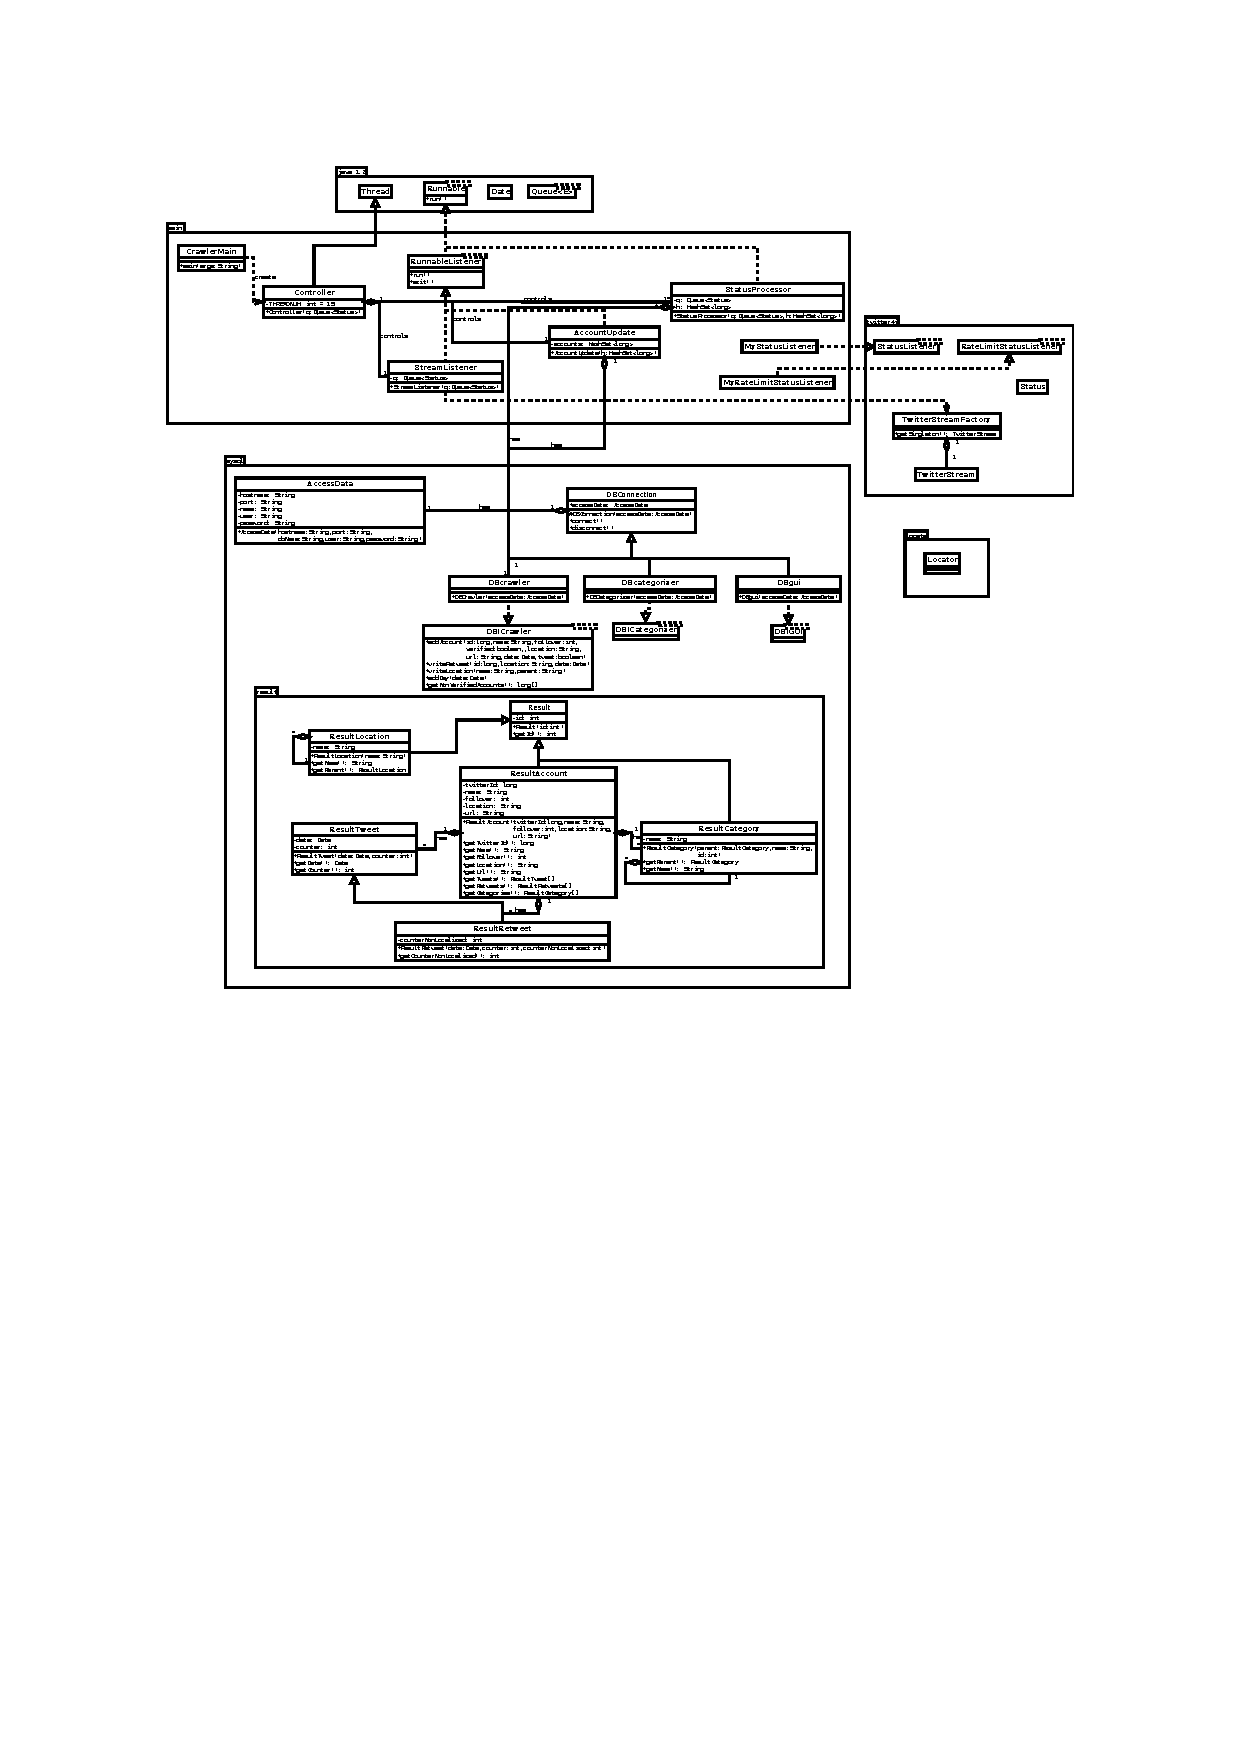
\includegraphics[width=\textwidth]{dia/uml_crawler}
\caption{UML-Klassendiagramm des Crawlers}
\label{fig:uml_crawler}
\end{figure}

\begin{description}
\item[CrawlerMain] Klasse dient als Einstieg ins Programm. Sie überprüft die Eingabe für die Datenbankverbindung und startet einen Controller. Danach seht sie dem Benutzer über die Konsole zur Verfügung um das Programm zu überwachen.
\item[RunnableListener] Interface welches Runnable erweitert und zusätzlich noch eine exit-Methode fordert um Threads zu beenden.
\item[Controller] Diese Klasse koordiniert alle Aktionen die nötig sind um Daten bei Twitter abzuholen und in die Datenbank zu Schreiben. Dazu startet sie einen StreamListener, ein AccountUpdate und mehrere StatusProcessor's jeweils als Thread. Außerdem kontrolliert sie den Puffer und sorgt für ein sauberes Beenden des Programms indem alle Verbindungen ordnungsgemäß geschlossen und die Threads beendet werden.
\item[StreamListener] Stellt eine Verbindung zur Twitter-Streaming-API her und initialisiert einen MyStatusListener.
\item[AccountUpdate] Diese Klasse stellt eine Methode zur Verfügung um in der Datenbank periodisch nach Accounts zu suchen, welche manuell hinzugefügt wurden, aber auch wie Verifizierte behandelt werden sollen.
\item[StatusProcessor] Diese Klasse stellt die Funktionalität zur Filterung der Daten von Twitter zur Verfügung, welche sie aus dem Puffer nimmt. Außerdem bietet sie die Möglichkeit diese Daten in die Datenbank zu schreiben.
\item[MyStatusListener] Diese Klasse nimmt die Daten von Twitter entgegen und schreibt diese in einen Puffer.
\item[MyRateLimitStatusListener] Diese Klasse nimmt Meldungen von Twitter bezüglich RateLimits entgegen.
\item[Locator] Der Locator lokalisiert Accounts und Retweets mithilfe eines Webdienstes.
\end{description}

\section{Kategorisierer}

Der Kategorisierer wird in regelmäßigen Abständen vom Betriebssystem gestartet und verbindet sich mit der Datenbank. Über die Datenbankschnittstelle ließt er die bislang unkategorisierten Twitteraccounts aus Accountstabelle aus und sucht in der DMOZ-Datenbank nach passenden Kategorien. Diese werden dann in die Kreuztabelle AccountCategory eingetragen.

Im Diagramm \cref{fig:categorizer} ist der grundlegende Aufbau des Kategorisierers dargestellt:
\begin{figure}[htb]
	\includegraphics[width=\textwidth]{dia/categorizer}
	\caption{Klassendiagramm des Kategorisierers}
	\label{fig:categorizer}
\end{figure}

\section{GUI}

